% !TEX root = ../main.tex
\begin{frame}\begin{center}
\LARGE\textbf{Example}
\end{center}\end{frame}
%-------------------------------------------------------------------------------
%-------------------------------------------------------------------------------
\begin{frame}\textbf{Seminal paper}\vspace{0.3cm}
\begin{itemize}
\item \bibentry{Keane.1994}
\end{itemize}
\end{frame}
%-------------------------------------------------------------------------------
%-------------------------------------------------------------------------------
\begin{frame}\textbf{Model of occupational choice}\vspace{0.3cm}

\begin{itemize}\setlength\itemsep{1em}
\item 1,000 individuals starting at age 16
\item life cycle histories \medskip
\begin{itemize}\setlength\itemsep{1em}
\item school attendance
\item occupation-specific work status
\item wages
\end{itemize}
\end{itemize}
\end{frame}
%-------------------------------------------------------------------------------
%-------------------------------------------------------------------------------
\begin{frame}

  \begin{align*}
  \text{\textbf{Labor market}}\qquad\quad & \\
  & \\
  r_t(s_t, 1) =  w_{1t} = \exp\{& \underbrace{\alpha_{10}}_{\text{endowment}} + \underbrace{\alpha_{11} g_t}_{\text{schooling}} + \underbrace{\alpha_{12}e_{1t} + \alpha_{13}e^2_{1t}}_{\text{own experience}} \\
              & + \underbrace{\alpha_{14}e_{2t} + \alpha_{15}e^2_{2t}}_{\text{other experience}} + \underbrace{\epsilon_{1t}}_{\text{shock}}\}
  \end{align*}
  \end{frame}
%-------------------------------------------------------------------------------
%-------------------------------------------------------------------------------
\begin{frame}

\begin{align*}
\text{\textbf{Schooling}} & \\
& \\
r_t(s_t, 3) = & \underbrace{\beta_0}_{\text{taste}} - \underbrace{\beta_1 \Ind[\,g_t \geq 12\,]}_{\text{direct cost}} - \underbrace{\beta_2\Ind[\,a_{t - 1} \neq 3\,]}_{\text{reenrollment effort}} + \underbrace{\epsilon_{3t}}_{\text{shock}} \\
& \\
\text{\textbf{Home}}\qquad & \\
& \\
r_t(s_t, 4) = & \underbrace{\gamma_0}_{\text{taste}} + \underbrace{\epsilon_{4t}}_{\text{shock}}
\end{align*}
\end{frame}
%-------------------------------------------------------------------------------
%-------------------------------------------------------------------------------
\begin{frame}

\textbf{State space}\vspace{0.3cm}
\begin{align*}
	s_t = \{g_t,e_{1t},e_{2t},a_{t - 1},\epsilon_{1t},\epsilon_{2t},\epsilon_{3t},\epsilon_{4t}\}
\end{align*}

\end{frame}
%-------------------------------------------------------------------------------
%-------------------------------------------------------------------------------
\begin{frame}
  \textbf{Transitions}\vspace{0.5cm}
\begin{itemize}
\item observed state variables
\begin{align*}
    e_{1,t+1} &= e_{1t} + \Ind[\,a_t = 1\,] \\
    e_{2,t+1} &= e_{2t} + \Ind[\,a_t = 2\,] \\
    g_{t+1}   &= g_{t\phantom{2}}    +  \Ind[\,a_t = 3\,]\\
\end{align*}
\item unobserved state variables
\begin{align*}
\{\epsilon_{1t},\epsilon_{2t},\epsilon_{3t},\epsilon_{4t}\} \sim N(0, \Sigma)
\end{align*}
\end{itemize}
\end{frame}
%-------------------------------------------------------------------------------
%-------------------------------------------------------------------------------
%\begin{frame}
%  \begin{figure}
%  \caption{Choices over the life cycle}\label{Choices over the life cycle}
%  \scalebox{0.35}{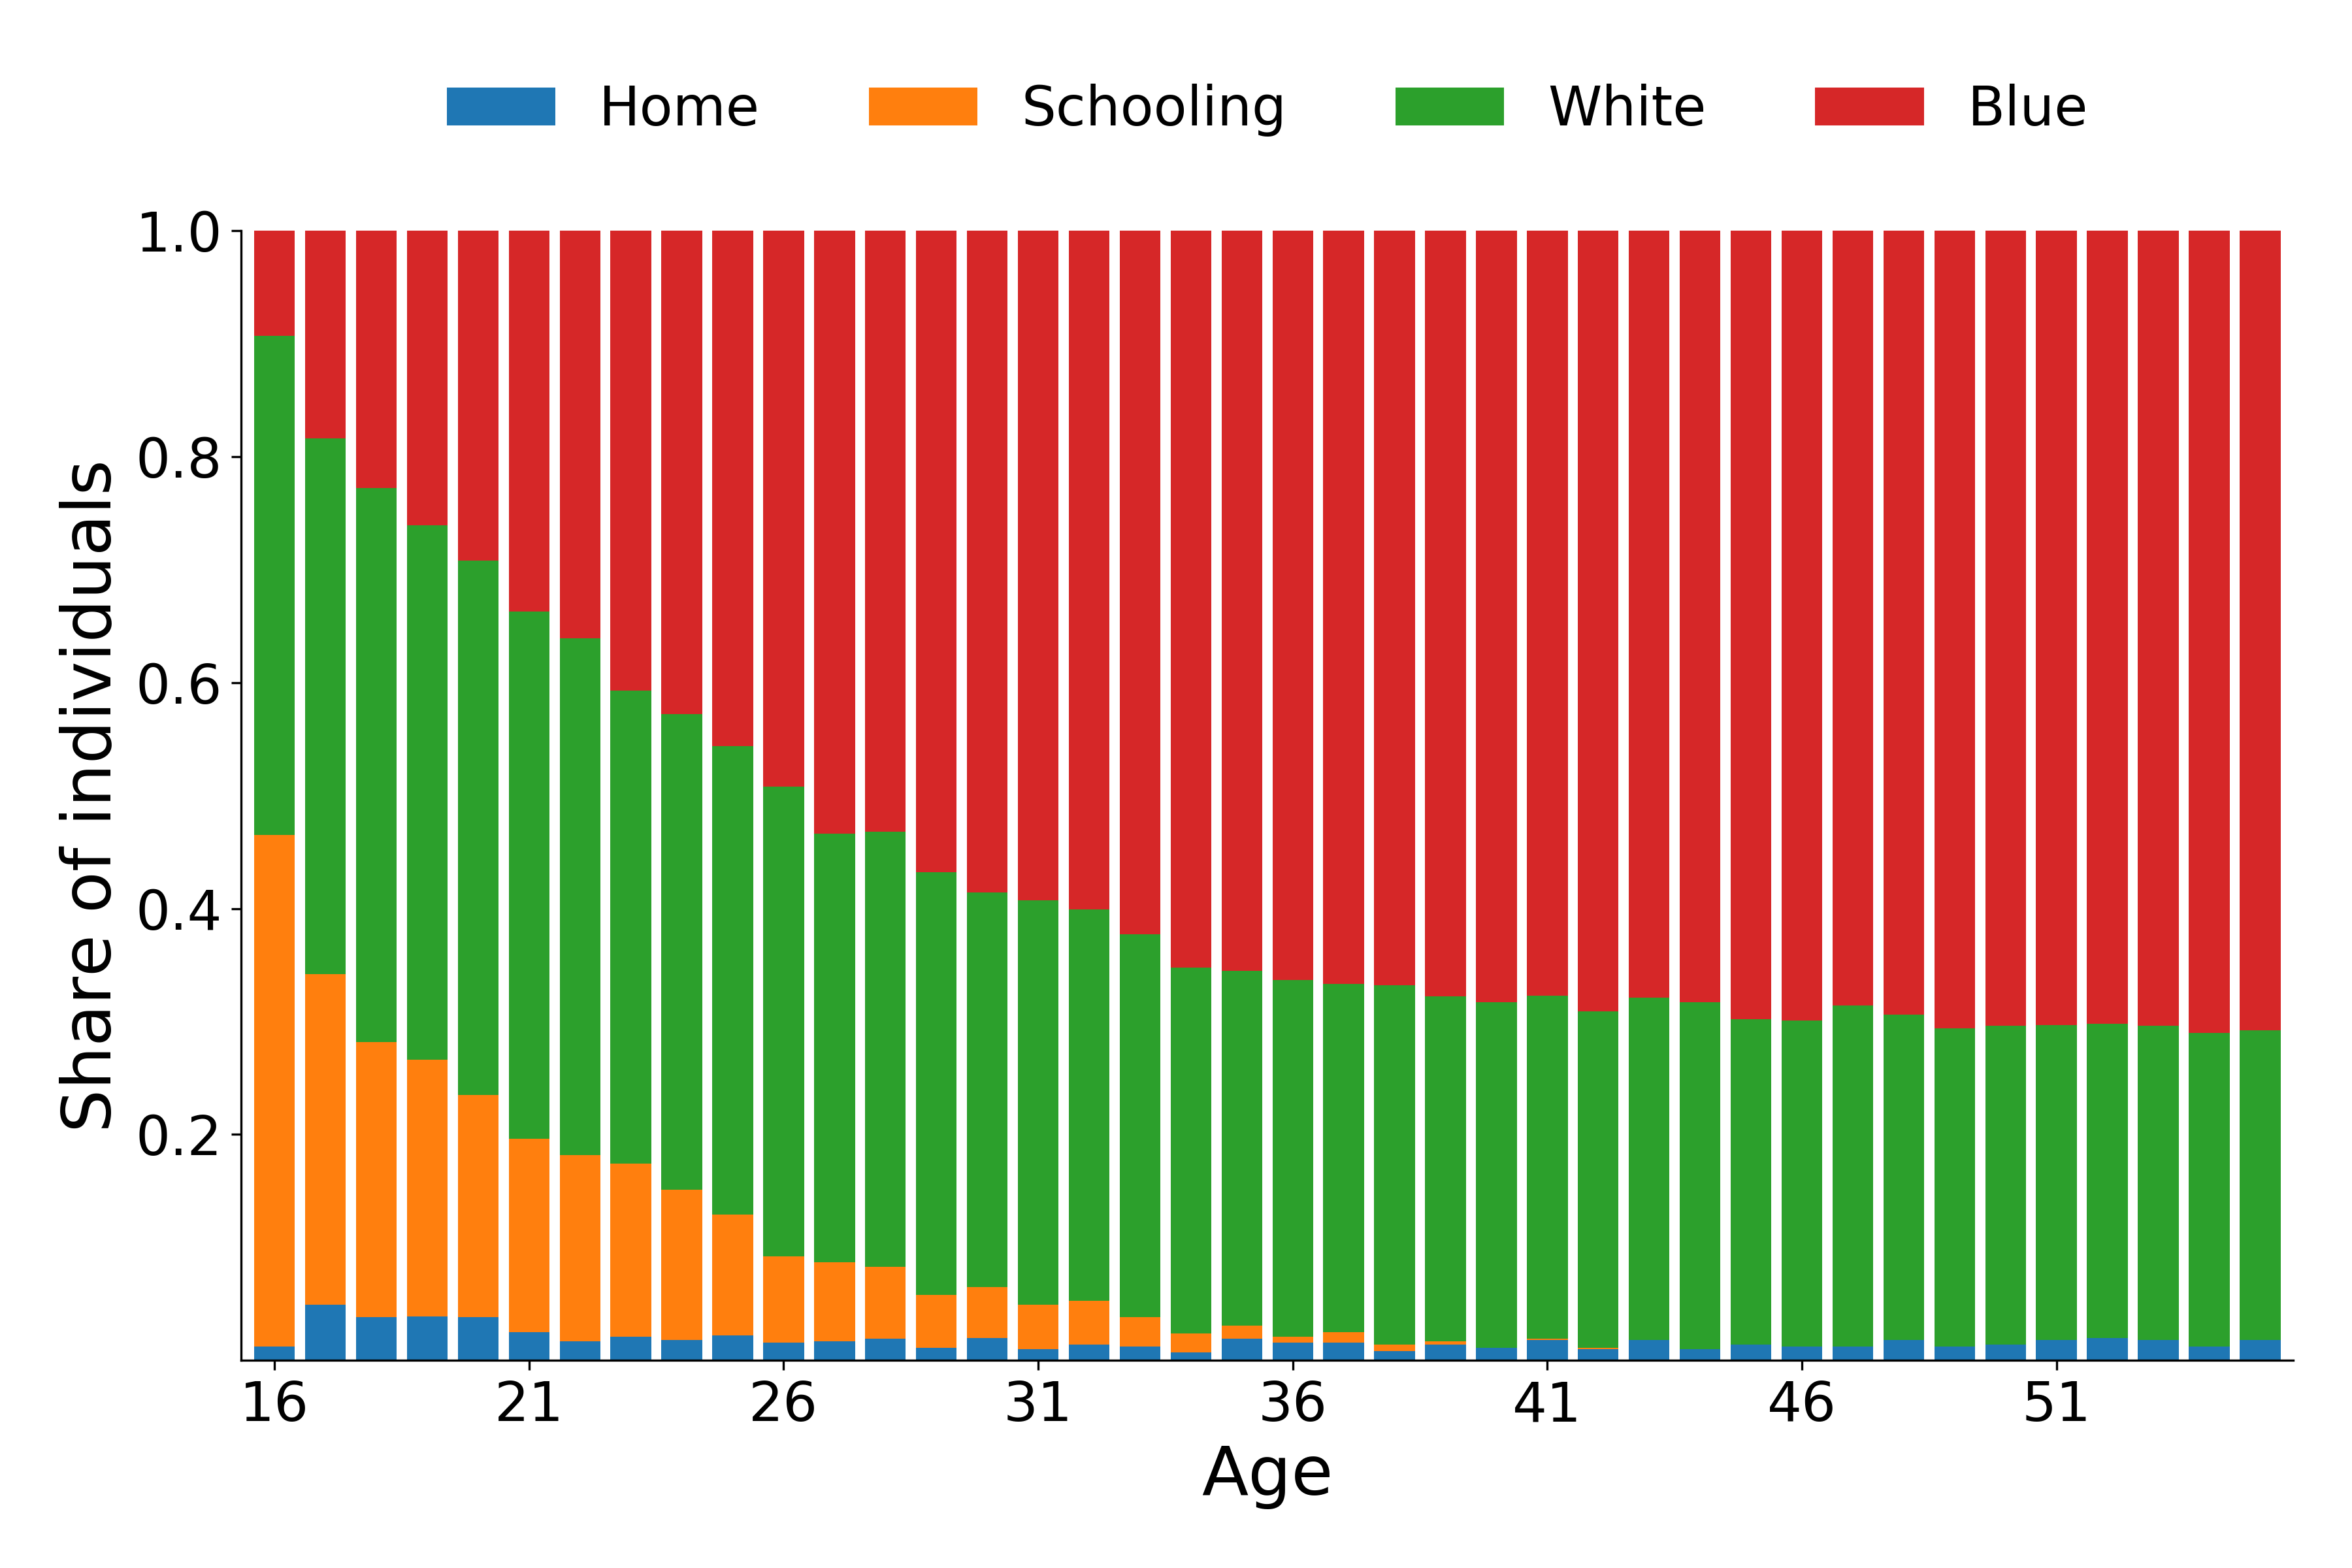
\includegraphics{fig-observed-choices}}
%  \end{figure}
%\end{frame}
%-------------------------------------------------------------------------------
%-------------------------------------------------------------------------------
%\begin{frame}
%  \begin{figure}[h!]\centering
%  \caption{Economic mechanism and policy forecast}\label{Economic mechanism and policy forecast}
%  \subfloat[Time preference]{\scalebox{0.15}{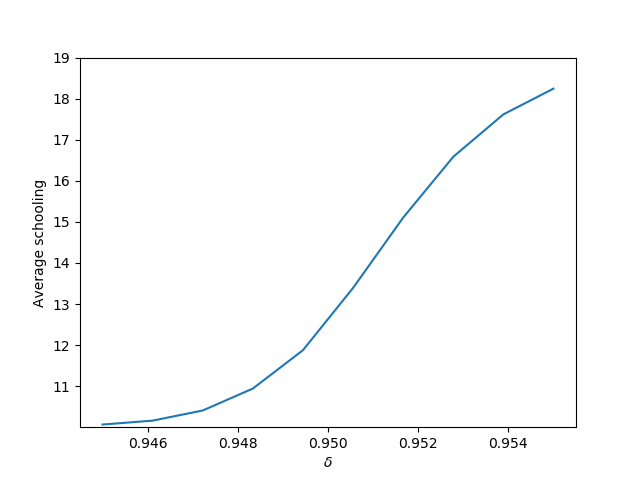
\includegraphics{fig-economic-mechanisms}}}\hspace{0.3cm}
%  \subfloat[Tuition subsidy]{\scalebox{0.15}{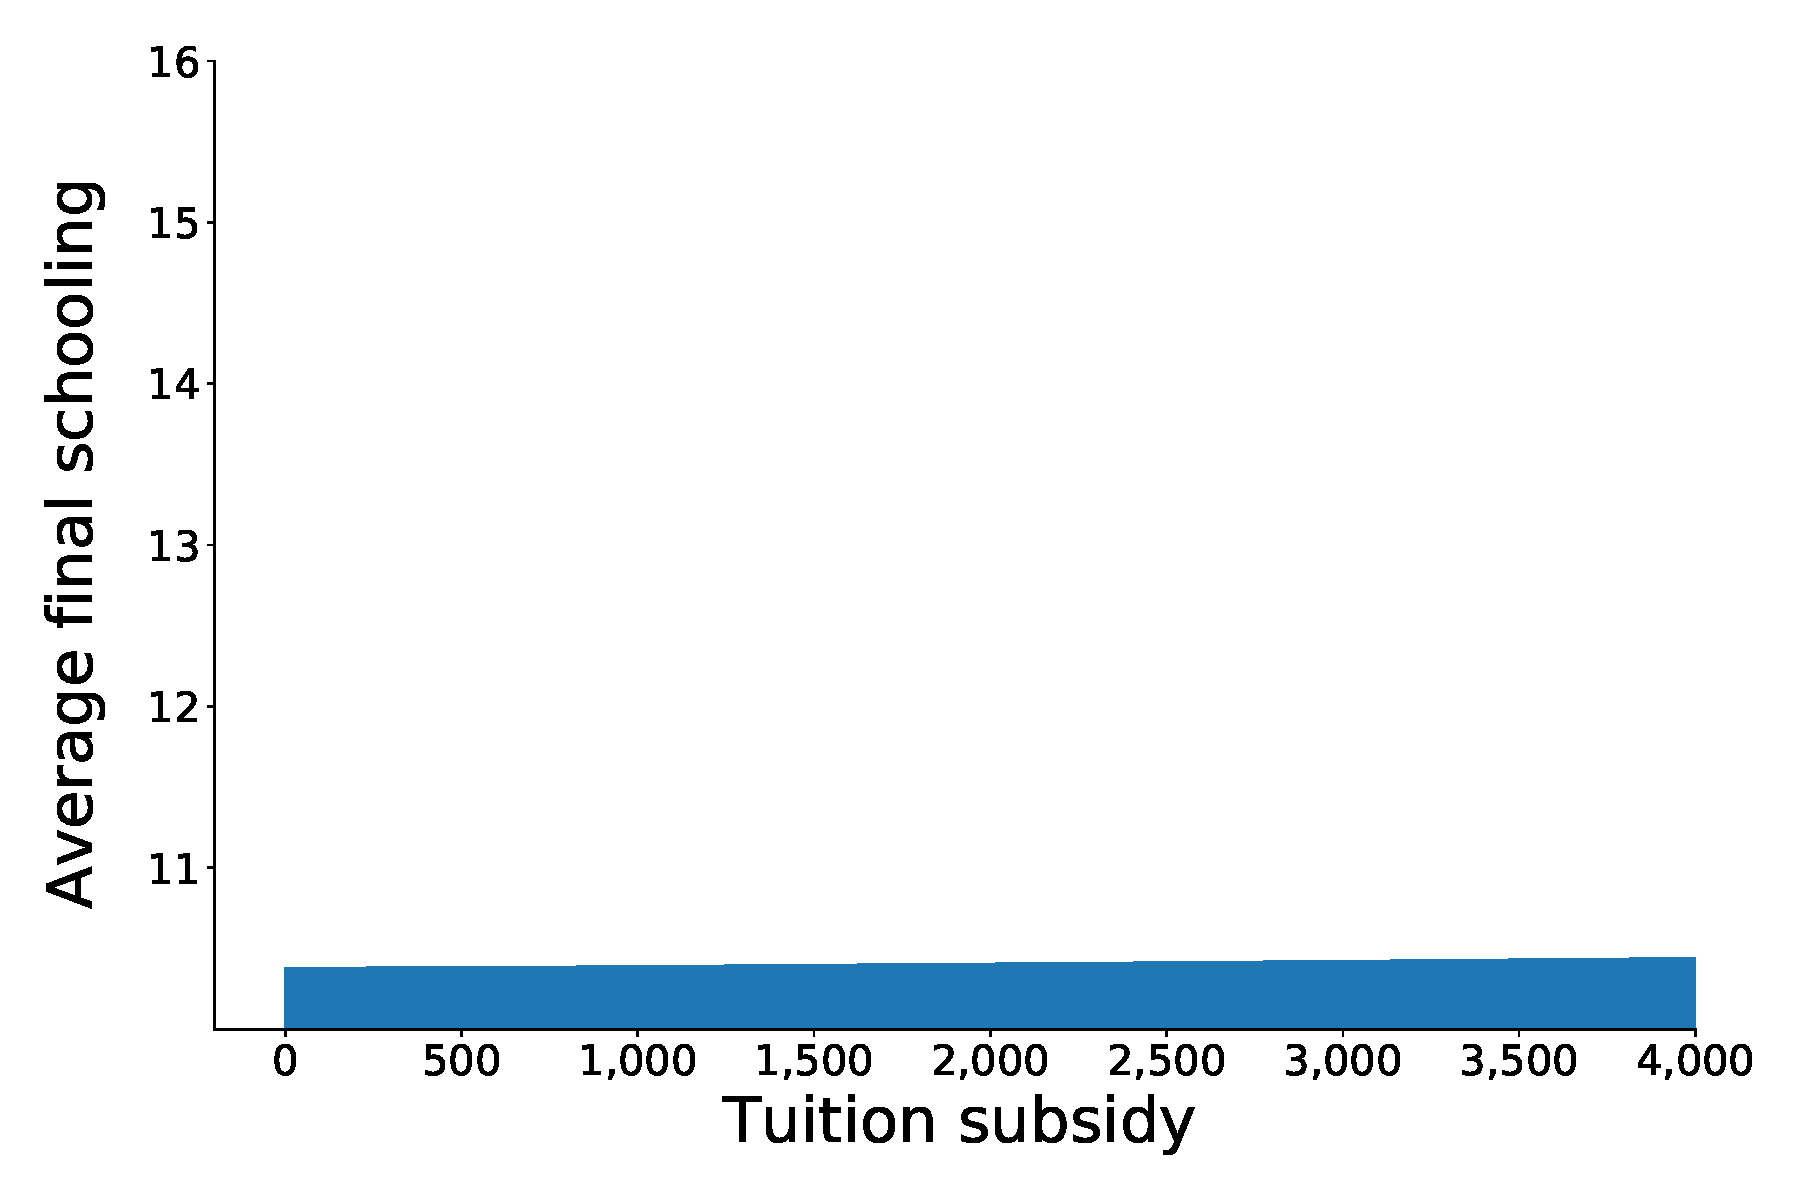
\includegraphics{fig-policy-forecast}}}
%  \end{figure}
%\end{frame}
%-------------------------------------------------------------------------------
%-------------------------------------------------------------------------------
\begin{frame}\begin{center}
  \Large\textit{Research codes}
\end{center}\end{frame}
%-------------------------------------------------------------------------------
%-------------------------------------------------------------------------------
\begin{frame}
\textbf{respy}\\\vspace{0.3cm}
\begin{tabular}{ll}
GitHub  & \url{OpenSourceEconomics/respy}\\
Docs    & \url{respy.readthedocs.io}\\
\end{tabular}\\\vspace{1cm}

\textbf{estimagic}\\\vspace{0.3cm}
\begin{tabular}{ll}
GitHub	& \url{OpenSourceEconomics/estimagic}\\
Docs    & \url{estimagic.readthedocs.io}\\
\end{tabular}

\end{frame}
%-------------------------------------------------------------------------------
%-------------------------------------------------------------------------------
\begin{frame}
  \begin{figure}\tiny
    \caption{Typical workflow}
   \lstset{language=python, morekeywords={as}, ndkeywords={=}, ndkeywordstyle=\color{blue}, keywordstyle=\color{red}, commentstyle=\color{darkgrey}, emph={get_example_model, get_crit_func, get_simulate_func}, emphstyle=\color{violet}}
         \lstinputlisting{../material/workflow.py}
   \end{figure}
\end{frame}
%-------------------------------------------------------------------------------
%-------------------------------------------------------------------------------
\begin{frame}

  \begin{figure}[h!]\centering
  \caption{Model specification}\label{Model specification}
  \subfloat[Parameterization]{\scalebox{0.28}{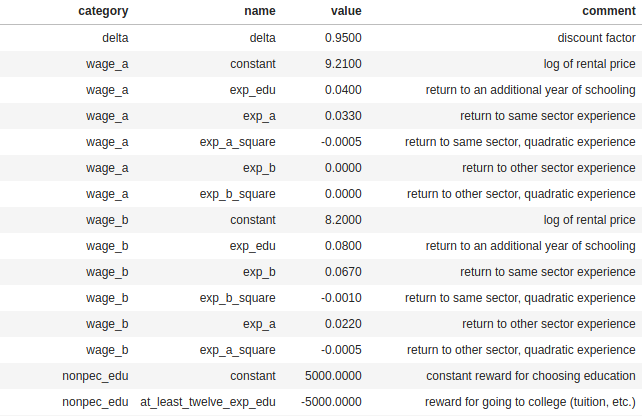
\includegraphics{params}}}\hspace{0.3cm}
  \subfloat[Options]{\scalebox{0.28}{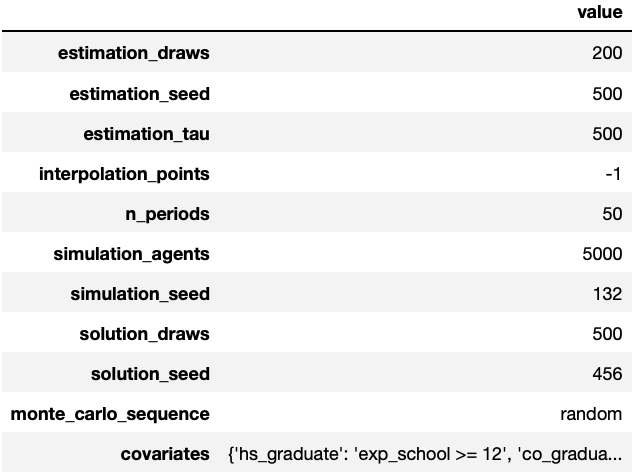
\includegraphics{options}}}
  \end{figure}

\end{frame}
%-------------------------------------------------------------------------------
%-------------------------------------------------------------------------------
\begin{frame}

  \begin{figure}[h!]\centering
  \caption{Dashboard}\label{Dashboard}
  \scalebox{0.50}{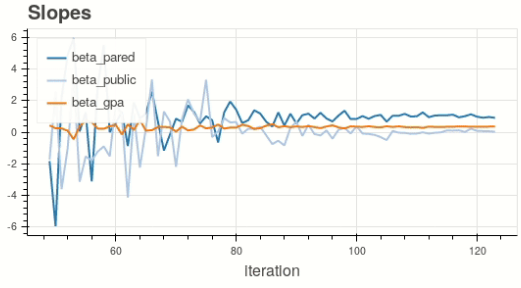
\includegraphics{crop-dashboard}}
  \end{figure}

\end{frame}
%-------------------------------------------------------------------------------
%-------------------------------------------------------------------------------
